\scanpage{83}
% Archive pencil foliation: 82.
est muni d'un élément \inserted{$\handwritten{\underline}{f}_q$} de $G_{\deleted{a}\handwritten{\nu}}(K_{\deleted{a}\handwritten{\nu}})$\inserted{(\handwritten{``}Frobenius relatif à $\handwritten{\underline}{F}_q$'')}\handwritten{\begin{tikzpicture}[baseline=0cm,x=1cm,y=1cm]\draw[thin] (0,-.15)..controls (-.08,.1) and (.1,.18)..(.23,.18)--(3.5,.18)..controls (3.6,.17) and (3.7,.28)..(3.66,.38);\end{tikzpicture}}. Ce dernier n'est autre d'ailleurs que $\deleted{\handwritten{\underline}{f}_q}$ $\handwritten{\underline}{f}^{\deleted{a}\handwritten{\nu}}$, où $\handwritten{\underline}{f}$ est le générateur canonique de $G$ (le Frobenius \unsure{\deleted{l}a|\deleted{d}a|\deleted{a}l|\deleted{a}d}bsolu \handwritten{!}). \deleted{\unsure{O|Q|C} on voit donc que $G_a$ est encore engendré par} Notons que $a\operatorname{\unsure{\deleted{i}I|\deleted{l}I|\deleted{I}i|\deleted{I}l}d}_G$ est un monomorphis\unsure{\deleted{e}m|\deleted{m}e}\unsure{\deleted{d}e|\deleted{r}e|e|\deleted{e}d|\deleted{e}r}. (car \begin{tikzcd}[cramped]x\arrow[r,no head,to path={(\tikztostart)--(\tikztotarget) (\tikztostart)++(0,-2pt)--++(0,4pt) (\tikztotarget)++(0,-1.8pt)--++(0,2.5pt)\tikztonodes}]&x^{\deleted{a}\handwritten{\nu}}\end{tikzcd} est un épimorphisme dans $\handwritten{\overline}{\handwritten{\underline}{Q}}_{\handwritten{p}}^{\handwritten{*}}$ ), donc \unsure{\deleted{x}i|\deleted{i}x}nduit un isomorphisme entre $G_{K_{\deleted{a}\handwritten{\nu}}}$ et $\unsure{\deleted{K}G|\deleted{G}K}_{\deleted{a}\handwritten{\nu}}\handwritten{\simeq}G(\handwritten{\underline}{F}_q)$,trans\unsure{\deleted{o}f|\deleted{f}o}\unsure{\deleted{f}o|\deleted{o}f}rmant le frobenius \deleted{relati} absolu en le frobenius relatif à $\handwritten{\underline}{F}_q$. Grâce à ceci, on voit :

\handwritten{\uline}{Proposition} 10.1. La catégorie \inserted{tann.}\handwritten{\begin{tikzpicture}[baseline=0cm,x=1cm,y=1cm]\draw[thin] (0,-.15)..controls (-.08,.1) and (.1,.18)..(.23,.18)--(0.8,.18)..controls (0.9,.17) and (1.0,.28)..(0.9600000000000001,.38);\end{tikzpicture}} $\operatorname{Fcriso}(\handwritten{\underline}{F}_q)\handwritten{\otimes}_{\overset{\mathrm{Fr.}}{\handwritten{\underline}{Q}}_p}K_a$ est équivalente à la catégorie \inserted{tann.}\handwritten{\begin{tikzpicture}[baseline=0cm,x=1cm,y=1cm]\draw[thin] (0,-.15)..controls (-.08,.1) and (.1,.18)..(.23,.18)--(0.8,.18)..controls (0.9,.17) and (1.0,.28)..(0.9600000000000001,.38);\end{tikzpicture}} $\operatorname{Fcriso}(\handwritten{\underline}{F}_p)\handwritten{\otimes}_{\handwritten{\underline}{Q}_p}K_a$,\handwritten{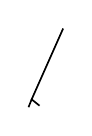
\begin{tikzpicture}[baseline=-.02cm,x=1cm,y=1cm]\draw[semithick] (.4,.9)--(0,0)--(.1,-.08);\draw[semithick] (0,0)--(-.04,-.1);\end{tikzpicture}} \margin{\handwritten{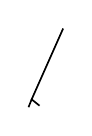
\begin{tikzpicture}[baseline=-.02cm,x=1cm,y=1cm]\draw[semithick] (.4,.9)--(0,0)--(.1,-.08);\draw[semithick] (0,0)--(-.04,-.1);\end{tikzpicture}}\handwritten{i.e. la catégorie des couples $(E,F'_E)$ d'un vectoriel sur $K_\nu$ et d'un autom de ce vectoriel....)}}
avec $\handwritten{\underline}{f}_q$ correspondant à $\handwritten{\underline}{f}^{\deleted{a}\handwritten{\nu}}$ (où on peut, si on veut, considérer $\handwritten{\underline}{f}_q$ et $\handwritten{\underline}{f}$ comme des end\unsure{\deleted{m}o|\deleted{n}o|\deleted{o}m|\deleted{o}n}\unsure{\deleted{E}m|\deleted{F}m|\deleted{h}m|m|\deleted{m}E|\deleted{m}F|\deleted{m}h}orphismes des foncteurs identiques de $\operatorname{Fcriso}(\handwritten{\underline}{F}_q)$ resp. $\operatorname{Fcriso}(\handwritten{\underline}{F}_p)$)), et corres\deleted{p}pondance des foncteurs fibres canoniques. Le foncteur déduit du ch\unsure{\deleted{n}a|\deleted{e}a|\deleted{a}n|\deleted{a}e}\unsure{\deleted{a}n|\deleted{e}n|\deleted{n}a|\deleted{n}e}gement de base \begin{tikzcd}[cramped]\handwritten{\underline}{F}_p\arrow[r]&\handwritten{\underline}{F}_q\end{tikzcd}

\diagram{\begin{tikzcd}
\operatorname{Fcriso}(\handwritten{\underline}{F}_{\unsure{\deleted{g}p|\deleted{q}p|p|\deleted{p}g|\deleted{p}q}})\handwritten{\otimes}_{\overset{\mathrm{Fr.}}{\handwritten{\underline}{Q}}_p}K_{\deleted{a}\handwritten{\nu}}\arrow[r]&\operatorname{Fcriso}(\handwritten{\underline}{F}_q)\handwritten{\otimes}_{\handwritten{\underline}{Q}_p}K_{\deleted{a}\handwritten{\nu}}
\end{tikzcd}}
\unsure{\deleted{n}s|\deleted{e}s|\deleted{a}s|s|\deleted{s}n|\deleted{s}e|\deleted{s}a}'identifie, par l'équivalence précédente, au foncteur qui à \unsure{tout|\deleted{o}tut|\deleted{t}out} couple $(E,F_E)$ d'un vectoriel sur $K_{\deleted{a}\handwritten{\nu}}$ et d'un automorphisme dudit, associe le couple $(E,F_E{}^{\deleted{a}\handwritten{\nu}})$\handwritten{;}
\inserted{\handwritten{analogue \unsure{p\textsuperscript{r}|pour} \begin{tikzcd}[cramped]\operatorname{Fcriso}(F_{\unsure{1|q}})\arrow[r,no head]&\operatorname{Fcriso}(\underline{F}_q)\otimes_{\mathbb{Q}_p}K_\nu\end{tikzcd}, \unsure{il|Il} s'identifie : \begin{tikzcd}[cramped](E,F_E)\arrow[r,maps to]&(E,F_E{}^\nu)\end{tikzcd}.}}

10.2. Comme on connait $\handwritten{\underline}{G}(\handwritten{\underline}{F}_q)$ comme une sous-gerbe $\handwritten{\underline}{G}_{\deleted{a}\handwritten{\nu}}$ de $\handwritten{\underline}{G}=\handwritten{\underline}{G}(\handwritten{\underline}{F}_p)$, et que celle-ci contient $\handwritten{\underline}{H}$, on connait donc en principe \unsure{\deleted{d}l|\deleted{l}d}'inclusion
\diagram{\begin{tikzcd}
\handwritten{\underline}{H}\arrow[r]&\handwritten{\underline}{G}_{\deleted{a}\handwritten{\nu}}=\handwritten{\underline}{G}(F_q)\quad ,
\end{tikzcd}}
donc aussi le foncteur
\diagram{\begin{tikzcd}
\operatorname{Rep}(\handwritten{\underline}{G}_{\deleted{a}\handwritten{\nu}})\handwritten{\simeq}\operatorname{Fcriso}(\handwritten{\underline}{F}_q)\arrow[r,no head,to path={(\tikztostart)--(\tikztotarget) (\tikztotarget)++(-1pt,0) [fill] ..controls +(0,1.4pt) and +(0,1.4pt)..++(2pt,0)--cycle\tikztonodes}]&\operatorname{Rep}(\handwritten{\underline}{H})\quad\unsure{;|,}
\end{tikzcd}}
\deleted{\inserted{et} Considérons le foncteur correspondant}
\[
\deleted{\operatorname{\unsure{\deleted{R}F|\deleted{K}F|F|\deleted{F}R|\deleted{F}K}criso}(\handwritten{\underline}{F}_q)\handwritten{\otimes}_{\handwritten{\underline}{Q}_p}K_{\underset{\deleted{\unsure{a|q}}}{a}}\quad\operatorname{Rep}(\handwritten{\underline}{H})\handwritten{\otimes}_{\handwritten{\underline}{Q}_p}K_a\ .}
\]
\figure{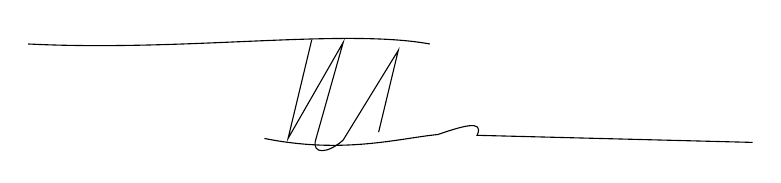
\begin{tikzpicture}[x=1cm,y=1cm]\draw[thin] (0,1.3)..controls (2,1.2) and (4,1.5)..(5.1,1.3);\draw[thin] (3.6,1.35)--(3.3,.1)--(4,1.32)--(3.65,.08)..controls (3.6,-.1) and (3.8,-.1)..(4,.08)--(4.7,1.22)--(4.45,.18);\draw[thin] (3,.1)..controls (4,-.1) and (4.7,.1)..(5.2,.15)..controls (5.5,.25) and (5.8,.35)..(5.7,.14)--(9.2,.05);\end{tikzpicture}}
L'effet de ce\deleted{s} foncteur\deleted{s} sur les classes d'isomorphie d'éléments est connu (comme chaque fois qu'il s'agit d'un morphisme d'une \deleted{gerbe de} \unsure{\deleted{O}c|\deleted{C}c|\deleted{c}O|\deleted{c}C}atégorie tannakienne à lien commutatif dans une autre à lien de type multiplicatif) par la connaiss\unsure{\deleted{n}a|\deleted{e}a|\deleted{a}n|\deleted{a}e}\unsure{\deleted{a}n|\deleted{o}n|\deleted{n}a|\deleted{n}o}\unsure{c|e}e de l'homomorphisme de liens correspondant

